\documentclass[border=5mm]{standalone}
\usepackage{tikz}
\usetikzlibrary{decorations.pathmorphing}
\usepackage[siunitx]{circuitikz}

\begin{document}
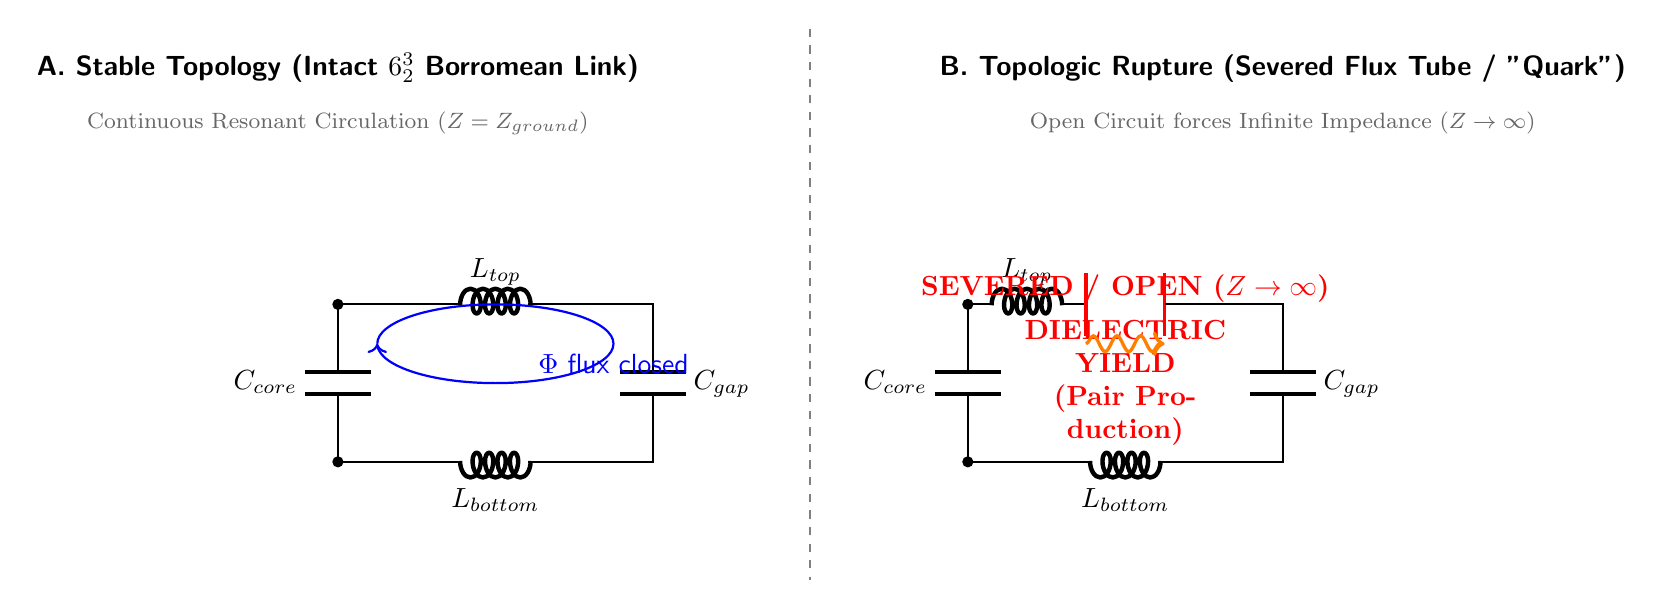
\begin{tikzpicture}[font=\sffamily, thick]
    
    % Panel 1: Intact Topology (Stable Proton)
    \node at (0, 3) {\textbf{A. Stable Topology (Intact $6^3_2$ Borromean Link)}};
    \node at (0, 2.3) [text=black!60, font=\footnotesize] {Continuous Resonant Circulation ($Z = Z_{ground}$)};
    
    % Left side network
    \draw (0, 0)
        to[L, l=$L_{top}$] (4, 0)
        to[C, l=$C_{gap}$] (4, -2)
        to[L, l=$L_{bottom}$] (0, -2)
        to[C, l=$C_{core}$, *-*] (0, 0);
        
    \draw[->, blue, thick] (0.5, -0.5) arc (180:-180:1.5 and 0.5) node[midway, below] {$\Phi$ flux closed};
    
    % Separation line
    \draw[dashed, gray] (6, 3.5) -- (6, -3.5);
    
    % Panel 2: Severed Topology (Deep Inelastic Scattering)
    \node at (12, 3) {\textbf{B. Topologic Rupture (Severed Flux Tube / "Quark")}};
    \node at (12, 2.3) [text=black!60, font=\footnotesize] {Open Circuit forces Infinite Impedance ($Z \to \infty$)};
    
    \draw (8, 0)
        to[L, l=$L_{top}$] (9.5, 0); 
        
    \node[red, font=\bfseries] at (10, 0.2) {SEVERED / OPEN ($Z \to \infty$)};
    \draw[red, very thick] (9.5, 0.4) -- (9.5, -0.4);
    \draw[red, very thick] (10.5, 0.4) -- (10.5, -0.4);
    
    \draw (10.5, 0)
        to[short] (12, 0)
        to[C, l=$C_{gap}$] (12, -2)
        to[L, l=$L_{bottom}$] (8, -2)
        to[C, l=$C_{core}$, *-*] (8, 0);
        
    \node at (10, -1) [red, text width=3cm, align=center, font=\bfseries] {DIELECTRIC YIELD \\ (Pair Production)};
    
    % Spark indicator for vacuum bridging
    \draw[orange, ->, very thick, decorate, decoration={snake, amplitude=1mm, segment length=3mm}] (9.5, -0.5) -- (10.5, -0.5);

\end{tikzpicture}
\end{document}
